%% $\stmt \in \Stmt$ &::= & $\skipstmt \mid \assert{le} \mid $ \\
%%                   & & $\call{A} \mid \call{P} \mid \async{P} \mid $\\
%%                   & & $s;\;s \mid \yield{e} \mid \ablock{e}{s} \mid$\\
%%                  & & $\ite{\locExpr}{s}{s} \mid$ \\
%%                   & & $\while{e}{\locExpr}{s}$ \\ 

\newcommand{\FH}[3]{\{#1\} #2 \{#3\}}
\newcommand{\re}{\mathit{re}}
\newcommand{\RM}{\mathit{RM}}
\newcommand{\CM}{\mathit{CM}}
\newcommand{\LM}{\mathit{LM}}

\begin{figure}
\scriptsize{
\medskip
%%%%%%%%%%%%%%%%%%%%
$
\inferrule
{
}
{P \jr \skipstmt : \epsilon}
\;(\textsc{Skip})
$
\medskip
%%%%%%%%%%%%%%%%%%%%
$
\inferrule
{
}
{P \jr \assert{\locExpr} : \epsilon}
\;(\textsc{Assert})
$
\medskip
%%%%%%%%%%%%%%%%%%%%
$
\inferrule
{
\mov(P') \neq \perp \\ \act(P') \Rightarrow \havoc{H}
}
{P \jr \call{P'} : \epsilon}
\;(\textsc{Call-Loop})
$
\medskip
%%%%%%%%%%%%%%%%%%%%
$
\inferrule
{
\mov(P') \neq \perp \\ \act(P') \Rightarrow \act{P}
}
{P \jr \ablock{e}{s} : A}
\;(\textsc{Call-Action})
$
\medskip
%%%%%%%%%%%%%%%%%%%%
$
\inferrule
{
\mov(P') \neq \perp \\ \act(P') \Rightarrow \havoc{H}
}
{P \jr \async{P'} : \epsilon}
\;(\textsc{Async})
$
\medskip
%%%%%%%%%%%%%%%%%%%%
$
\inferrule
{
\jp \FH{e}{s}{\havoc{H \cup L}}
}
{P \jr \ablock{e}{s} : \epsilon}
\;(\textsc{Ablock-Loop})
$
\medskip
%%%%%%%%%%%%%%%%%%%%
$
\inferrule
{
\jp \FH{e}{s}{\act(P)}
}
{P \jr \ablock{e}{s} : A}
\;(\textsc{Ablock-Action})
$
\medskip
%%%%%%%%%%%%%%%%%%%%
$
\inferrule
{
P \jr s_1 : \re_1 \\ P \jr s_2 : \re_2
}
{P \jr s_1;s_2 : \re_1\cdot\re_2}
\;(\textsc{Seq})
$
\medskip
%%%%%%%%%%%%%%%%%%%%
$
\inferrule
{
P \jr s_1 : \re_1 \\ P \jr s_2 : \re_2
}
{P \jr \ite{\locExpr}{s_1}{s_2} : \re_1+\re_2}
\;(\textsc{Ite})
$
\medskip
%%%%%%%%%%%%%%%%%%%%
$
\inferrule
{
P \jr s : \re
}
{P \jr \while{e}{\locExpr}{s} : \re^*}
\;(\textsc{While})
$
\medskip
%%%%%%%%%%%%%%%%%%%%

}
\caption{Refinement rules}
\label{fig:refinement}
\end{figure}


\begin{figure}
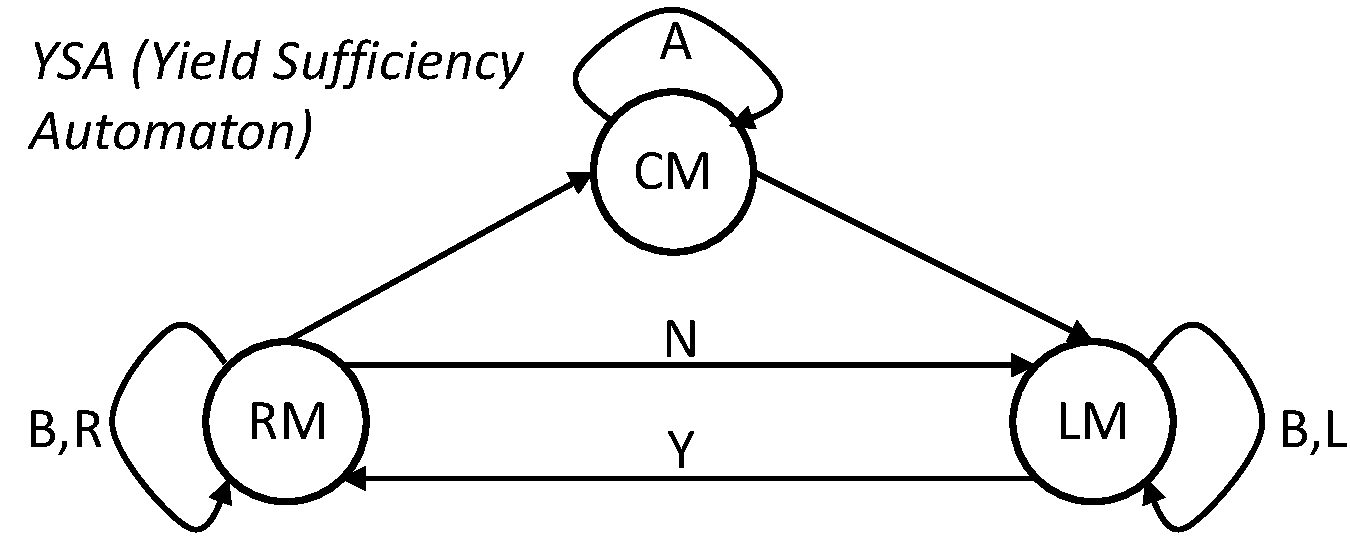
\includegraphics[scale=0.4]{YieldTypeCheckingAutomaton.pdf}
\caption{Specification for yield sufficiency}
\label{fig:YieldTypeCheckingAutomaton}
\end{figure}

\begin{figure}
\scriptsize{
\medskip
%%%%%%%%%%%%%%%%%%%%
$
\inferrule
{
}
{P \jy \skipstmt : x \leadsto x}
\;(\textsc{Skip})
$
\medskip
%%%%%%%%%%%%%%%%%%%%
$
\inferrule
{
}
{P \jy \assert{\locExpr} : x \leadsto x}
\;(\textsc{Assert})
$
\medskip
%%%%%%%%%%%%%%%%%%%%
$
\inferrule
{
\mov(P') = B
}
{P \jy \call{P'} : x \leadsto x}
\;(\textsc{CallBothMover})
$
\medskip
%%%%%%%%%%%%%%%%%%%%
$
\inferrule
{
\mov(P') = R
}
{P \jy \call{P'} : \RM \leadsto \RM}
\;(\textsc{CallRightMover})
$
\medskip
%%%%%%%%%%%%%%%%%%%%
$
\inferrule
{
\mov(P') = L
}
{P \jy \call{P'} : x \leadsto \LM}
\;(\textsc{CallLeftMover})
$
\medskip
%%%%%%%%%%%%%%%%%%%%
$
\inferrule
{
\mov(P') = N
}
{P \jy \call{P'} : \RM \leadsto \LM}
\;(\textsc{CallYield})
$
\medskip
%%%%%%%%%%%%%%%%%%%%
$
\inferrule
{
\mov(P') = \perp
}
{P \jy \call{P'} : x \leadsto \RM}
\;(\textsc{CallYield})
$
\medskip
%%%%%%%%%%%%%%%%%%%%
$
\inferrule
{
}
{P \jy \async{P'} : x \leadsto \LM}
\;(\textsc{Async})
$
\medskip
%%%%%%%%%%%%%%%%%%%%
$
\inferrule
{
x \in \{\RM,\CM\}
}
{P \jy \ablock{e}{s} : x \leadsto \CM}
\;(\textsc{Ablock})
$
\medskip
%%%%%%%%%%%%%%%%%%%%
$
\inferrule
{
P \jy s_1 : x \leadsto y \\ P \jy s_2 : y \leadsto z
}
{P \jy s_1;s_2 : x \leadsto z}
\;(\textsc{Seq})
$
\medskip
%%%%%%%%%%%%%%%%%%%%
$
\inferrule
{
P \jy s_1 : x \leadsto y \\ P \jy s_2 : x \leadsto y
}
{P \jy \ite{\locExpr}{s_1}{s_2} : x \leadsto y}
\;(\textsc{Ite})
$
\medskip
%%%%%%%%%%%%%%%%%%%%
$
\inferrule
{
P \jy s : x \leadsto x
}
{P \jy \while{e}{\locExpr}{s} : x \leadsto x}
\;(\textsc{While})
$
\medskip
%%%%%%%%%%%%%%%%%%%%

}
\caption{Yield sufficiency rules}
\label{fig:yield-sufficiency}
\end{figure}
